\section{Interest Flooding Attacks in NDN}
\label{sec:interest-flooding}



As we explained earlier, Interest packets in NDN are routed through the network based on content name prefixes and consume memory resources at intermediate routers. This makes them a potential tool to launch DDoS attacks in NDN. An attacker or a set of distributed attackers can inject excessive number of Interests in an attempt to overload the network and cause service disruptions for legitimate users (Fig.~\ref{fig:flooding example}). 

\begin{figure}[t]
  \centering
  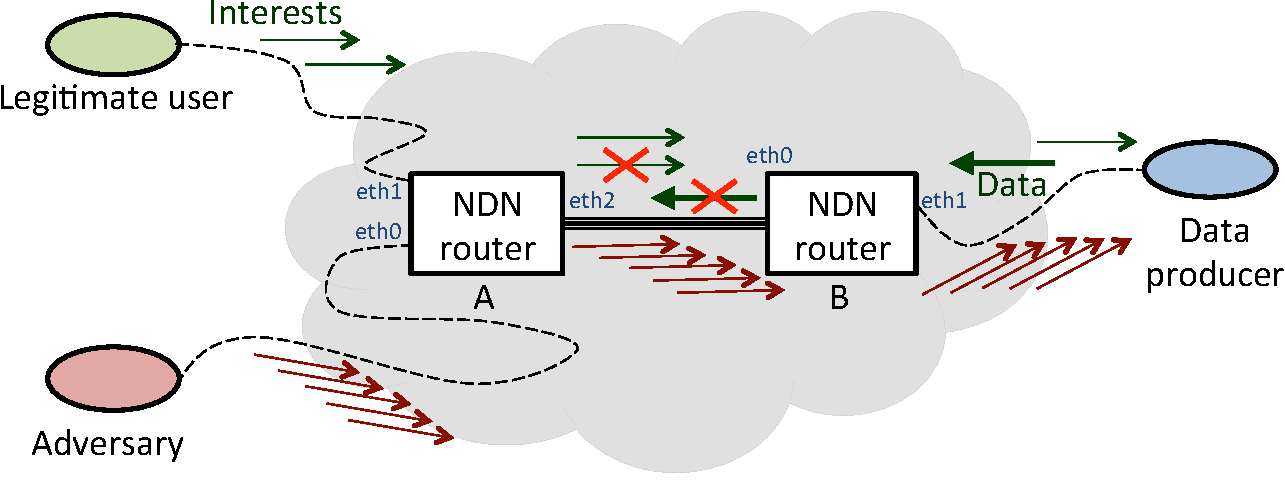
\includegraphics[scale=0.3]{attack-definition}
  \caption{Example of Interest flooding attack}
  \label{fig:flooding example}
  \vspace{-0.3cm}
\end{figure}


Since an NDN network fetches data by its name, an adversary cannot easily target specific routers or end-hosts.
However, an adversary can target a specific namespace.
For example in Fig.~\ref{fig:flooding example}, if the data producer is the exclusive owner of \ndnName{/foo/bar} namespace, both router B and the data producer would receive all Interests for \ndnName{/foo/bar/\ldots} that cannot be otherwise satisfied from in-network caches.%
\footnote {This example assumes that the adversary floods the network with unique data names carrying \ndnName{\small /foo/bar} prefix to make them effective. It also assumes the producer is single-homed and the data is not replicated elsewhere. With multi-homed producers or replicated data, NDN would likely to cope better with DDoS attacks due its native multipath and adaptive forwarding~\cite{adaptive-forwarding, Yi:2013:A-Case-for-Stateful} support.}
A large volume of such malicious Interests can disrupt service quality in NDN network in two ways: \emph{create network congestion} and \emph{exhaust resources on routers}.

Similar to packets in traditional networks, Interest packets in NDN consume a portion of network capacity. A large number of Interest packets might cause congestion and lead to legitimate packets being dropped in the network. In particular, a coordinated DDoS attack could target one specific namespace and concentrate attack traffic in certain segments of the network, as routing in NDN is based on name prefixes. 


As NDN routers maintain per-packet states for each forwarded Interest (i.e., an entry in its PIT), an excessive amount of malicious Interests can lead to exhaustion of a router's memory, making the router unable to create new PIT entries for incoming Interests and disrupting service for legitimate users.

Nevertheless, creating an effective Interest flooding attack in NDN is non-trivial.
To efficaciously target a specific namespace (e.g., \ndnName{/newyorktimes/}), an adversary needs to make sure that (1)~the expressed Interests are routed towards and as close to the data producer/provider as possible, and (2)~new corresponding PIT entries are created for those interests and are stored at intermediate NDN routers for as long as possible. The former is achieved when Interests share the same name prefix (e.g., \ndnName{/newyorktimes/}) and as long as they are not served from caches of intermediate routers---an Interest is not forwarded upstream if a router can satisfy it from its content store. The latter requires every single malicious Interest to ask for unique content---all Interests requesting the same content are combined into one PIT entry in routers. Thus, an adversary has to request either an unpopular (i.e., not cached in routers) or non-existing unique content with each Interest. Of the two options available to an adversary, the first one is challenging due to the difficulties around indexing content names in a particular namespace, coordinating a large number of bots to send unique Interests, and sustaining the attack while the network is continuously caching the requested content objects. However, the second option---requesting a unique non-existing content with each Interest---is easy to achieve and sustain. For example, an adversary can construct such Interests by concatenating a variable-length random name component to the victim namespace (e.g., \ndnName{/newyorktimes/3rf3...}). In this paper, we exclusively focus on this particular attack strategy as it not only maximizes the damage from each malicious Interest, but also is the one that is easy to launch and widely applicable to all namespaces (small or large). % other less effective strains of Interest flooding attacks can also be mitigated by applying the same or similar countermeasures described in the next section.  

In the rest of this paper, we use the general term \emph{Interest flooding attack} to refer to the above described attack and assume an attacker is limited to controlling a botnet of end-hosts only, i.e., we assume the routers in the network and the computers in the victim domain are not compromised.

%\paragraph{Assumptions} 
%E: These are assumptions for the simulations on hand and particulary to test for the worst case scenario in many aspects. They are not the paper's assumption and in fact the paper first should be more general on describing all possibilities. Then it should explain the assumptions for the simulations and discuss why they make sense and do NOT favor positive results in some way. 

% - assumptions about attacker position
% - assumptions about the producer / producer namespace
% - assumptions about the attack traffic / attack pattern

%In this paper we are making the following assumptions about the Interest flooding attack:
%\begin{itemize}
%\item only client nodes can be compromised and become attack bots;
%\item there are no colluding attackers inside the Data producer's network;
%\item the attack is carried only using unique junk Interests; and
%\item there is only one Data producer for the attacked prefix.
%\end{itemize}

%We also assume that NDN forwarding strategy uses only single-path Interest forwarding, always choosing the best-metric route advertised by the routing protocol.
%This way, we are able to analyze the attack in its best environment, as enabling the multi-path forwarding would only alleviate effects of the Interest flooding attack.

%In section~\ref{sec:discussion} we discuss potential of the Interest flooding attack under several other attack assumptions.
